
\section{Upper bound of $k_{\mathrm{c}}$}
\label{sec:bound_kc}
In this appendix, we prove that
\begin{align}
    \frac{k_{\mathrm{c}}}{\widetilde{N}}\leq K_{\mathrm{c}}+\frac{1}{2\widetilde{N}}+\frac{2\pi}{3\widetilde{N}^{2}},
\end{align}
where $K_{\mathrm{c}}$ is the limit of $k_{\mathrm{c}}/\widetilde{N}$.

We first derive $K_{\mathrm{c}}$. Setting $y=l/\widetilde{N}$ gives the continuum limit $\widetilde{N}\to\infty$ of $s_{k}/\widetilde{N}$ as
\begin{align}
    &t(x) = \int_{0}^{x}b(y)\diff y,\\
    &b(y) = -\cos2\pi y+\cos^{2}2\pi y.
\end{align}
Then $K_{\mathrm{c}}$ is given as the solution of the self-consistent equation;
\begin{align}
    8\pi t(K_{\mathrm{c}})=4\pi K_{\mathrm{c}}+\sin 4\pi K_{\mathrm{c}}-4\sin 2\pi K_{\mathrm{c}}=0.
\end{align}
Conventional search algorithms such as the binary search or the Newton--Raphson method give us an approximate value of $K_{\mathrm{c}}$ as $0.34046\cdots$.

To see the difference between $K_{\mathrm{c}}$ and $k_{\mathrm{c}}/\widetilde{N}$,
we calculate $s_{k}/\widetilde{N}$ as an equation deviated from $t(k/\widetilde{N})$. In the following, we restrict the range of $k$ to $1/4\leq k/\widetilde{N}\leq 1/2$ to focus on the value of $s_{k}/\widetilde{N}$ around $k=k_{\mathrm{c}}$. From a trigonometric identity
\begin{align}
    \sum_{l=0}^{k}\cos l\theta=\frac{\sin(k\theta)}{2\tan(\theta/2)}+\cos^{2}\left(\frac{k\theta}{2}\right),
\end{align}
we rewrite $s_{k}/\widetilde{N}$ as
\begin{align}
    \frac{s_{k}}{\widetilde{N}}=&\frac{1}{2}\frac{k}{\widetilde{N}}-\frac{1}{2\pi}\frac{\pi/\widetilde{N}}{\tan[\pi/\widetilde{N}]}\sin\left(2\pi\frac{k}{\widetilde{N}}\right)\\
    &+\frac{1}{8\pi}\frac{2\pi/\widetilde{N}}{\tan[2\pi/\widetilde{N}]}\sin\left(4\pi\frac{k}{\widetilde{N}}\right)\\
    &+\frac{1}{2\widetilde{N}}b\left(\frac{k}{\widetilde{N}}\right).
\end{align}
Using an inequality
\begin{align}
    \tan x \geq x + \frac{x^{3}}{3} \quad x\geq 0,
\end{align}
we have
\begin{align}
    \frac{s_{k}}{\widetilde{N}} > &\frac{1}{2}\frac{k}{\widetilde{N}}-\frac{1}{2\pi}\sin\left(2\pi\frac{k}{\widetilde{N}}\right)+\frac{1}{8\pi}\sin\left(4\pi\frac{k}{\widetilde{N}}\right)\\
    &+\frac{1}{2\widetilde{N}}b\left(\frac{k}{\widetilde{N}}\right)-\frac{\pi}{3N^{2}}+\frac{5\pi^{3}}{18 N^{4}}\\
    >& t\left(\frac{k}{\widetilde{N}}\right)+\frac{1}{2\widetilde{N}}b\left(\frac{k}{\widetilde{N}}\right)-\frac{\pi}{3N^{2}}.
\end{align}

Assume that $k\geq\widetilde{N}K_{\mathrm{c}}-1/2+2\pi/(3\widetilde{N})$.
Then, from the mean value theorem and the monotonicity of $b(x)$, we have
\begin{align}
    t(K_{\mathrm{c}})-t\left(K_{\mathrm{c}}-\frac{1}{2\widetilde{N}}+\frac{2\pi}{3\widetilde{N}^{2}}\right)
    <\left(\frac{1}{2\widetilde{N}}-\frac{2\pi}{3\widetilde{N}^{2}}\right)b(K_{\mathrm{c}}).
\end{align}
Since $t(K_{\mathrm{c}})=0$ and $b(x)\leq 2$,
\begin{align}
    t\left(K_{\mathrm{c}}-\frac{1}{2\widetilde{N}}+\frac{2\pi}{3\widetilde{N}^{2}}\right)
    > -\frac{1}{2\widetilde{N}}b(K_{\mathrm{c}})+\frac{4\pi}{3\widetilde{N}^{2}}.
\end{align}
Hence we have
\begin{align}
    \frac{s_{k}}{\widetilde{N}}
    >& -\frac{1}{2\widetilde{N}}b(K_{\mathrm{c}})+\frac{4\pi}{3\widetilde{N}^{2}}
    +\frac{1}{2\widetilde{N}}b\left(\frac{k}{\widetilde{N}}\right)-\frac{\pi}{3N^{2}}\\
    >& -\frac{1}{2\widetilde{N}}\left[b(K_{\mathrm{c}})-b\left(K_{\mathrm{c}}-\frac{1}{2\widetilde{N}}+\frac{2\pi}{3\widetilde{N}^{2}}\right)\right]+\frac{\pi}{\widetilde{N}^{2}}.
\end{align}
Using the mean value theorem again gives
\begin{align}
    b(K_{\mathrm{c}})-b\left(K_{\mathrm{c}}-\frac{1}{2\widetilde{N}}+\frac{2\pi}{3\widetilde{N}^{2}}\right)=\left(\frac{1}{2\widetilde{N}}-\frac{2\pi}{3\widetilde{N}^{2}}\right)b'(x),
\end{align}
for some $x\in(K_{\mathrm{c}}-1/2\widetilde{N}+2\pi/(3\widetilde{N}^{2}),K_{\mathrm{c}})$.
Since $b'(x)$ is less than $4\pi$,
we obtain an evaluation of $s_{k}/\widetilde{N}$ as
\begin{align}
    \frac{s_{k}}{\widetilde{N}}&>-\frac{2\pi}{\widetilde{N}}\left(\frac{1}{2\widetilde{N}}-\frac{2\pi}{3\widetilde{N}^{2}}\right)
    +\frac{\pi}{\widetilde{N}^{2}}=\frac{4\pi^{2}}{3\widetilde{N}^{3}}>0,
\end{align}
meaning that $s_{k}>0$ as long as $k\geq\widetilde{N}K_{\mathrm{c}}-1/2+2\pi/(3\widetilde{N})$. From this, the desired evaluation holds:
\begin{align}
    k_{\mathrm{c}}\leq\left\lceil\widetilde{N}K_{\mathrm{c}}-\frac{1}{2}+\frac{2\pi}{3\widetilde{N}}\right\rceil
    \leq \widetilde{N}K_{\mathrm{c}}+\frac{1}{2}+\frac{2\pi}{3\widetilde{N}},
    \label{eq:kc_bound}
\end{align}
Figure~\ref{fig:kc} shows $k_{\mathrm{c}}/\widetilde{N}$ together with the derived bound.

\begin{figure}
    \centering
    % 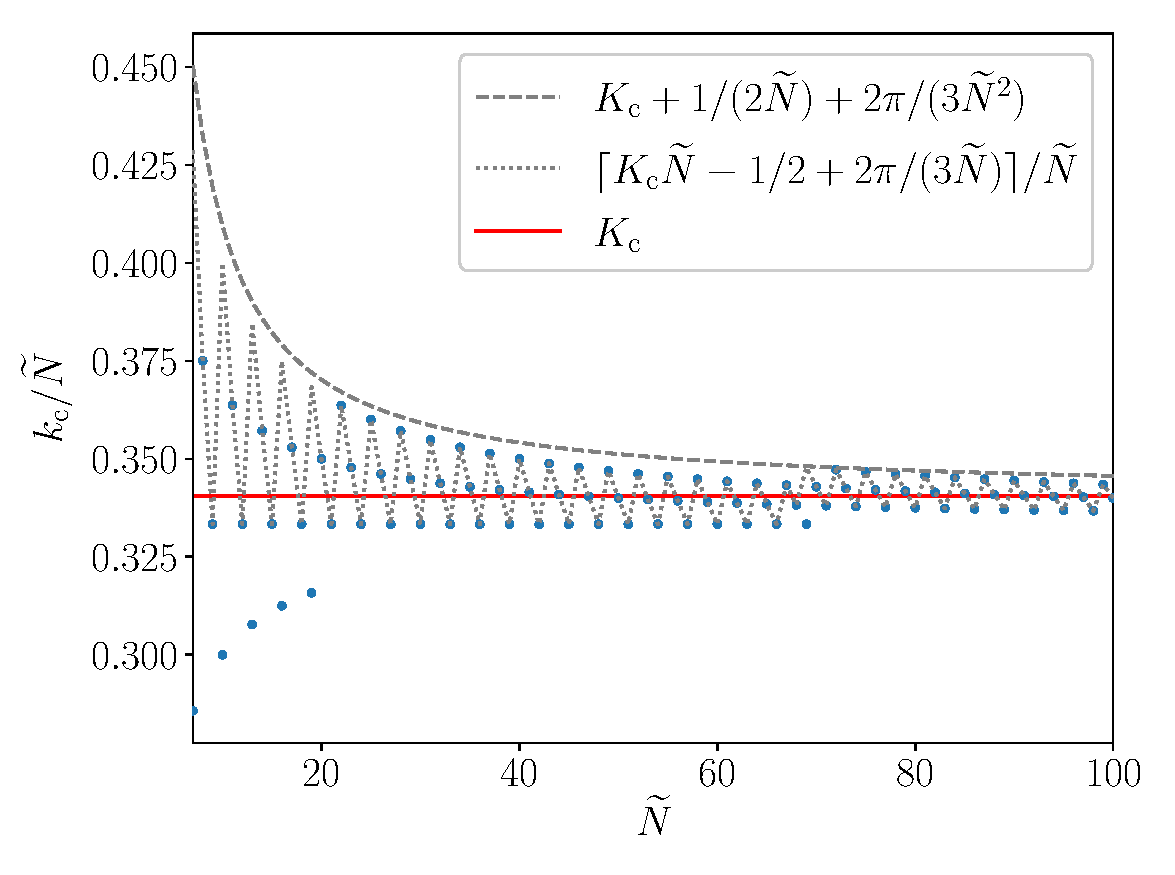
\includegraphics[width=8cm]{figs/kc.eps}
    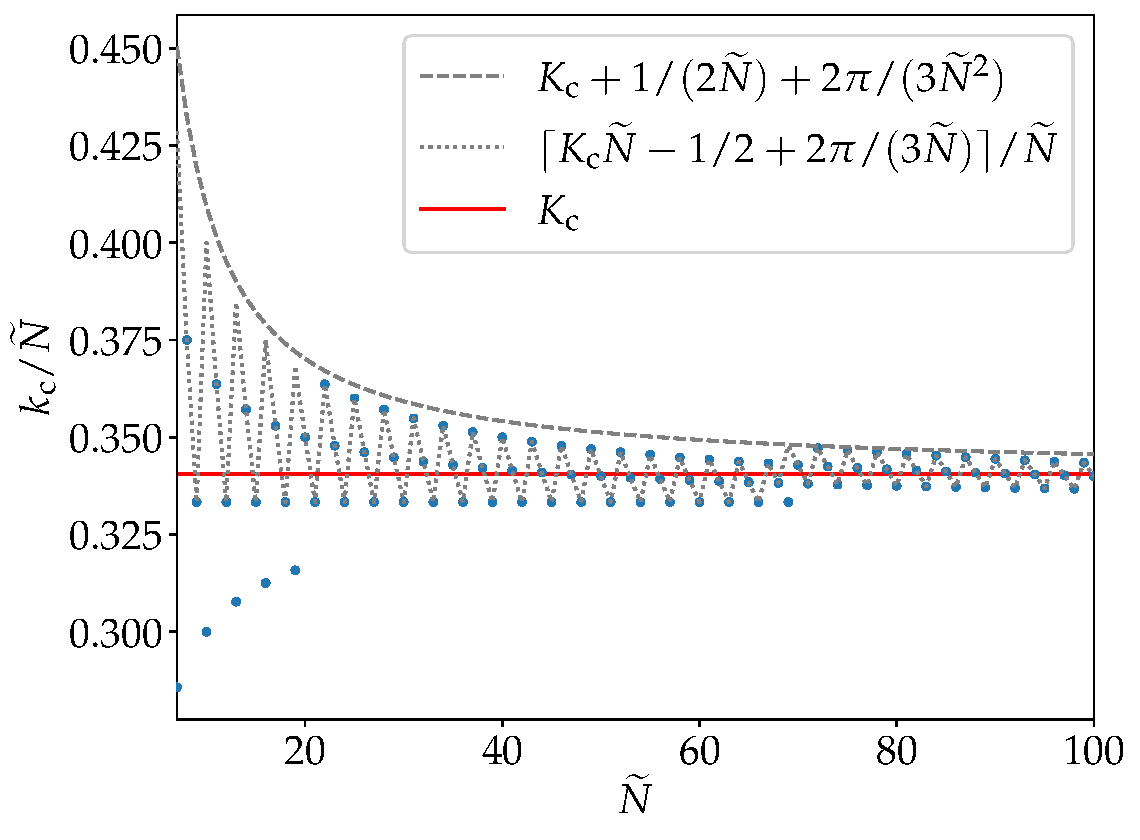
\includegraphics[width=0.7\textwidth]{figs/kc.pdf}
    \caption{
        $k_{\mathrm{c}}/\widetilde{N}$ for $7\leq\widetilde{N}\leq100$ together with the bound of $k_{\mathrm{c}}/\widetilde{N}$ obtained in \eqref{eq:kc_bound}.
        We see that $k_{\mathrm{c}}/\widetilde{N}$ gets close to $K_{\mathrm{c}}$ as $\widetilde{N}\to\infty$.
    }
    \label{fig:kc}
\end{figure}